\documentclass[12pt, titlepage]{article}
\usepackage[utf8]{inputenc}
\usepackage{amsmath,amsthm,amsfonts,amssymb,amscd}
\usepackage{multirow,booktabs}
\usepackage[table]{xcolor}
\usepackage{fullpage}
\usepackage{lastpage}
\usepackage{enumitem}
\usepackage{fancyhdr}
\usepackage{mathrsfs}
\usepackage{wrapfig}
\usepackage{setspace}
\usepackage{calc}
\usepackage{multicol}
\usepackage{cancel}
\usepackage[retainorgcmds]{IEEEtrantools}
\usepackage[margin=3cm]{geometry}
\usepackage{amsmath}
\newlength{\tabcont}
\setlength{\parindent}{0.0in}
\setlength{\parskip}{0.05in}
\usepackage{empheq}
\usepackage{framed}
\usepackage[most]{tcolorbox}
\usepackage{xcolor}
\colorlet{shadecolor}{orange!15}
\parindent 0in
\parskip 12pt
\geometry{margin=1in, headsep=0.25in}
\theoremstyle{definition}
\newtheorem{defn}{Definition}
\newtheorem{reg}{Rule}
\newtheorem{exer}{Exercise}
\newtheorem{note}{Note}

\usepackage[superscript,biblabel]{cite}
\usepackage{hyperref}
\hypersetup{colorlinks,linkcolor={blue},citecolor={blue},urlcolor={orange}}

\usepackage{graphicx}
% Path relative to the main .tex file
\graphicspath{ {./images/} }

\title{\textbf{Practical integrator using operational amplifier}}
\author{
  Russel Shawn Dsouza\\
  171EC143
  \and
  Sathvik S Prabhu\\
  171EC146
}
\date{}

\begin{document}
  % TODO Add NITK logo
  % TODO Add 'AIC Report' and date
  \maketitle

  \tableofcontents

  \newpage
  \section{Aim}
  To design, implement and test a $\mu$A741-based voltage integrator.


  \section*{Components required}
    \begin{itemize}
      \item $\mu$A741 OpAmp
      \item Resistors R = 120k$\Omega$, 3.3k$\Omega$, 4.7k$\Omega$
      \item Capacitor C= 0.01 $\mu$F
      \item Breadboard
      \item Digital Storage Oscilloscope
      \item Jumper wires
      \item Signal generator
    \end{itemize}


  \section*{Circuit diagram}
    % TODO Add circuit in LaTeX
    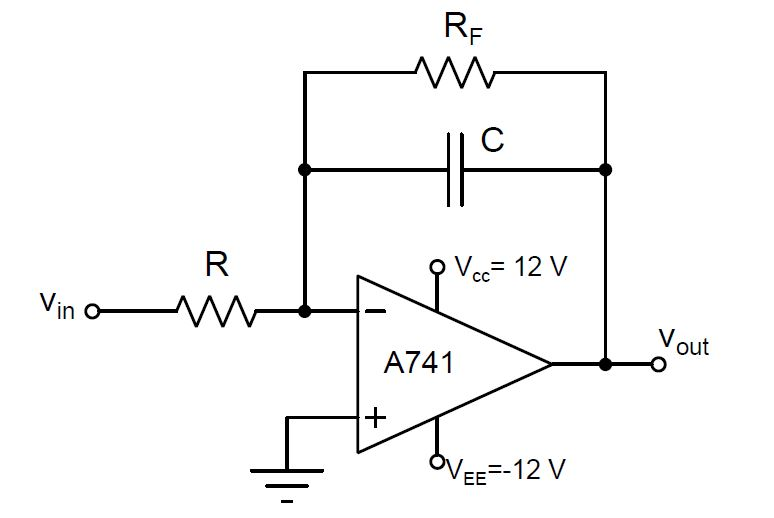
\includegraphics[scale=0.5]{circuit}\\
    % TODO Add captions and labels
    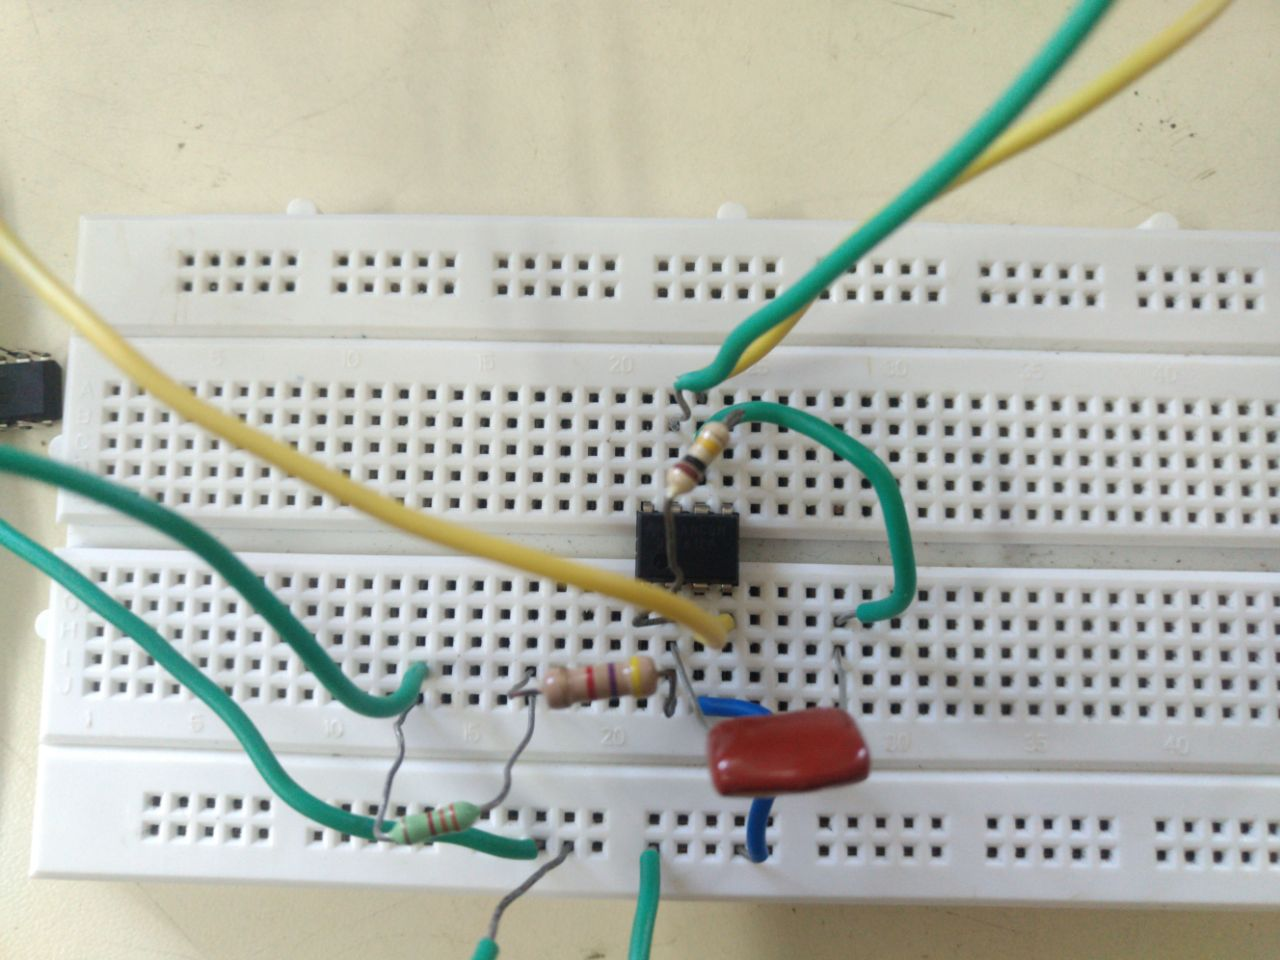
\includegraphics[scale=0.25]{practical_circuit}


  \newpage
  \section{Theory}
    % TODO Complete Theory
    In an integrator, the output voltage is proportional to the integral of the input.
    The response of an op amp circuit with feedback will reflect the characteristics of the feedback elements.
    In order to achieve integration, the feedback network can be constructed using a capacitor.

    In a practical integrator, one can overcome the limitations of an ideal integrator by adding resistor $R_{f}$ in parallel with capacitor C.
    This $R_{f}$ avoids op-amp going into open loop configuration at low frequencies.

    Frequency response of a practical integrator
    \begin{align*}
    H(s) &=\frac{-R_{F} || \frac{1}{Cs}}{R} \\
    H(j\omega)&=\frac{-R_{F}}{R} \left[ \frac{1}{1+R_{F}Cj\omega} \right] \\
    \end{align*}

    This gives,
    \begin{align*}
    |H(j\omega)|&=\frac{R_{F}}{R}\frac{1}{\sqrt{1+\omega^{2}R_{F}^{2}C^{2}}} \\
    \angle H(j\omega) &= \pi - tan^{-1}(\omega R_{F}C)
    \end{align*}


  \newpage
  \section{Design}
    % TODO Stepwise design
    Q. Design a $\mu$A741 based voltage integrator for a sinusoidal input $v_{in} = 2sin(4000\pi t)$.
    The integrator gain should be unity i.e. the output should have a peak to peak value same as that of the input.
    Also, it is required that the phase error should be kept below 5\%.
    Design the practical integrator with $f_{-3db} = \frac{f_{in}}{15}$.
    Make sure all resistances are of the order of k$\Omega$.


  \section{Calculations}
    % TODO Merge calculations with stepwise design
    Let $C=0.01\mu F$ , \\
    $f_{in}=2000 Hz$\\
    $f_{-3dB}=\frac{f_{in}}{15} = 133.33 Hz$ \\
    $\frac{1}{2\pi R_{F}C} = 133.33$\\
    $\frac{1}{2\pi RC} = 2000$\\
    $R=7.96k\Omega, R_{F}=119.37k\Omega$\\
    Expected DC gain= $\frac{R_{f}}{R}=15.25$\\
    Expected phase shift= $\frac{\pi}{2}=1.57 rad$


  \newpage
  \section{Simulation}
    % TODO Convert to white background images
    % TODO Add captions and labels
    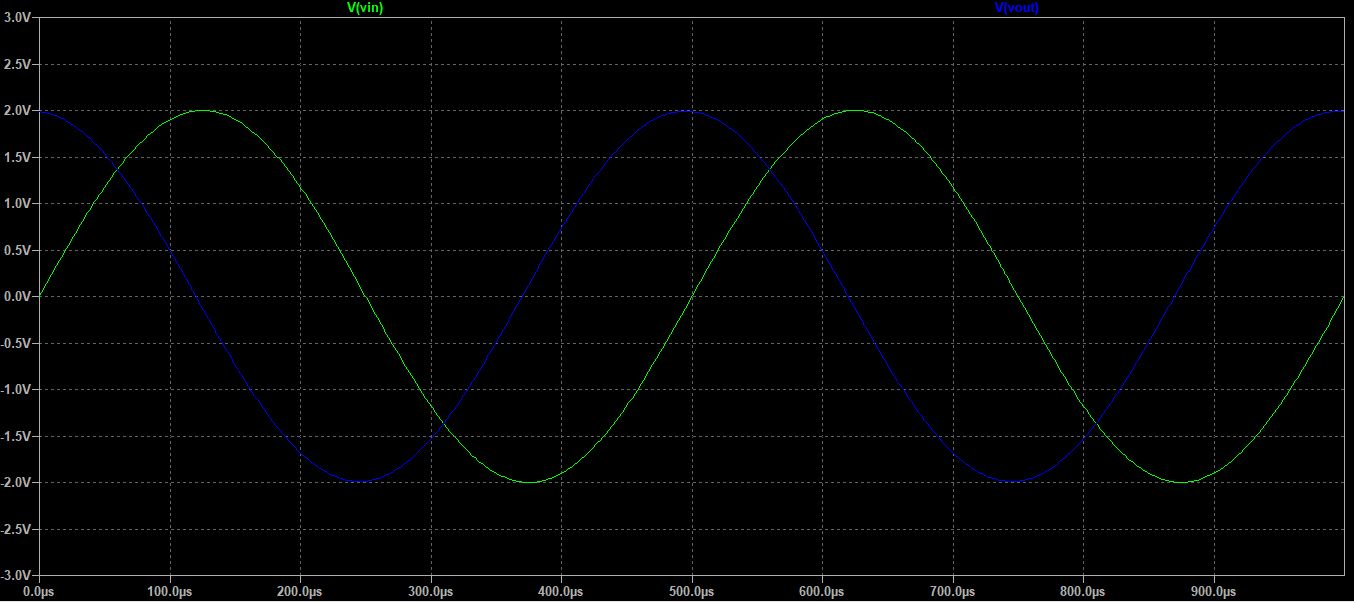
\includegraphics[width=\textwidth]{sim_plot1}
    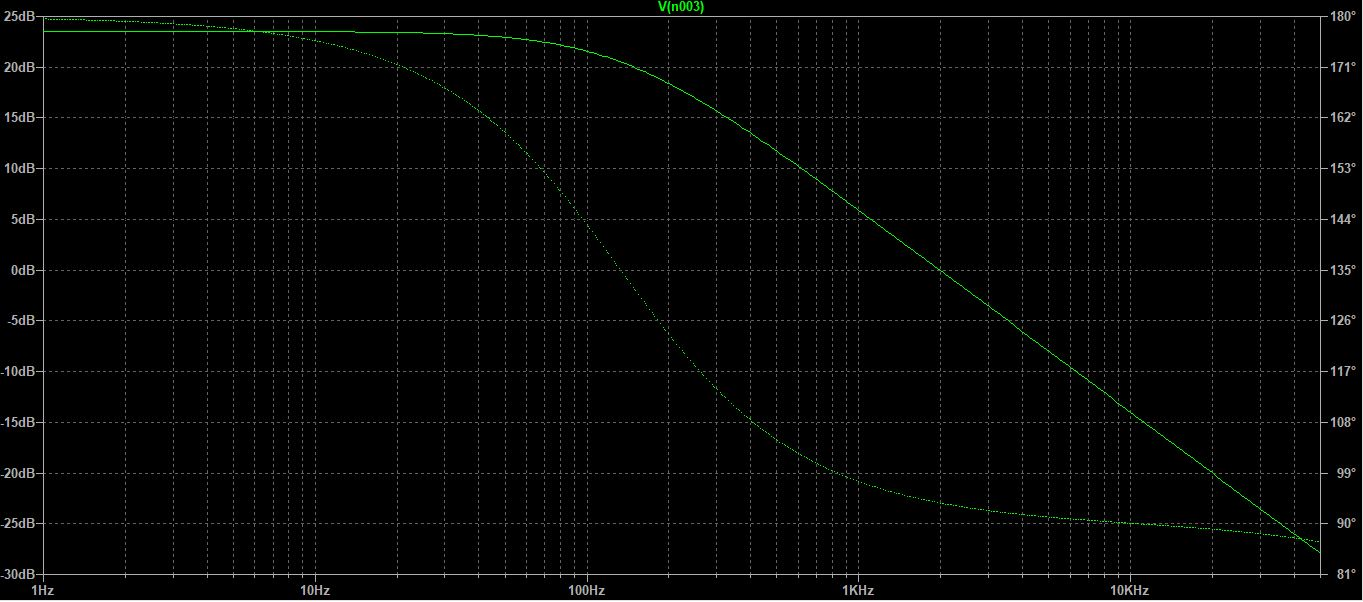
\includegraphics[width=\textwidth]{sim_plot2}

  % TODO Add a separate section for our implementation

  \newpage
  \section{Waveforms}
    % TODO Add captions and labels
    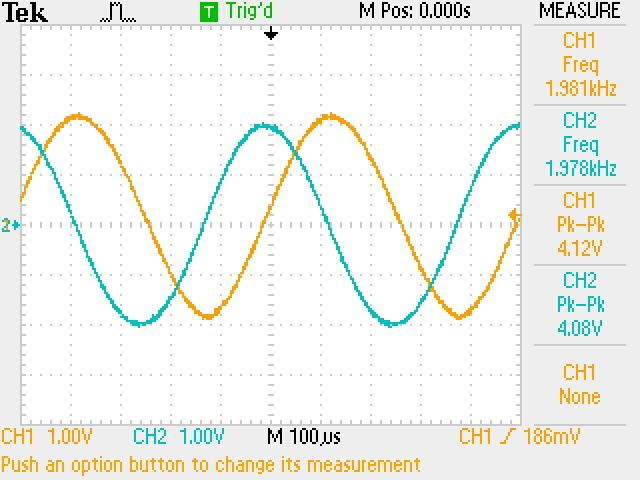
\includegraphics[width=\textwidth/2]{results_q1}
    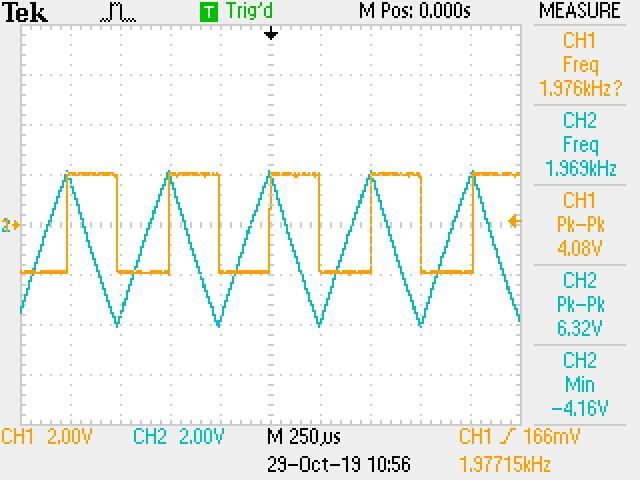
\includegraphics[width=\textwidth/2]{results_q3}
    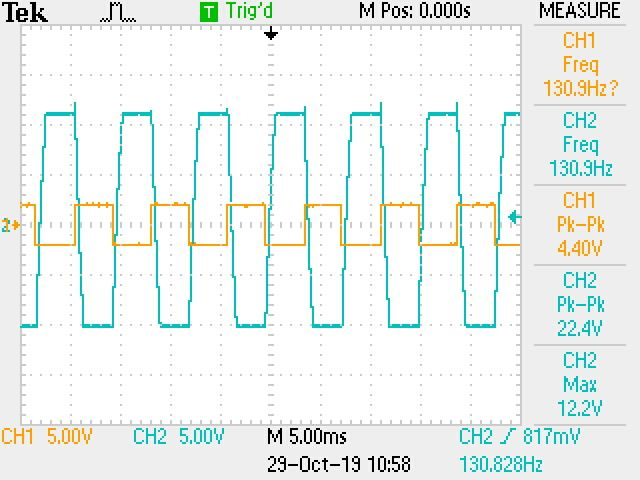
\includegraphics[width=\textwidth/2]{results_q4_2}


  \newpage
  \section{Observations}
    % TODO Convert from QnA to report format
    Q. Measure DC gain, -3dB frequency $f_{3dB}$, unity gain frequency $f_u$, roll-off rate and phase shift.

    % TODO Show calculation that was used to obtain these results
    \begin{itemize}
      \item[] DC gain = 14.89
      \item[] -3dB frequency = 132 Hz
      \item[] Unity gain frequency = 2.07 kHz
      \item[] Roll-off rate = -18.35 dB/decade
      \item[] Phase shift = 1.608 rad, an error of 2.4\%
    \end{itemize}

    Q. What happens if the feedback resistor $R_{F}$ is removed from the circuit? Give reasons.

    $V_{out}=\pm V_{sat}$ due to the capacitor acting as an open circuit at low frequencies. This sends the opamp into an open loop configuraton.

    Q. Apply a square wave of 4V peak-to-peak and frequency 2 kHz. What to you see and why?

    A triangular waveform is obtained as a result of the square wave being integrated.

    Q. Change the frequency of the square wave input to 130 Hz. What do you observe and why?

    The triangular waveform is now clipped at the $\pm V_{sat}$ levels.
    $C\Delta V=I\Delta V$
    Substituting $C=0.01\mu F$, $I=\frac{2}{8k}$, $t=\frac{0.5}{130}$,
    $\Delta V = 96.15 V$
    Since $\Delta V > 2V_{sat}$, $V_{out}$ gets clipped.


  \newpage
  \section{Results \& Conclusions}
    % TODO Add more results and better conclusions
    The $\mu$A741 based voltage integrator was designed and implemented successfully.
\end{document}
